\setcounter{chapter}{2}
\setcounter{section}{0}

\chapter{Dispositivi}
    \par
        Il CEGO offre diversi servizi informatici e multimediali, tra i quali è prevista la possibilità di condividere la schermata di un qualsiasi computer tramite un impianto multimediale ad hoc presente, in diverse misure, in tutte le aule che sono gestite dall'Ateneo\footnote{\cite{AuleMultimedialiVideotutorial}} permettendo così una maggiore fruizione del materiale didattico proposto da ciascun Docente, aumentando quindi l'accessibilità ai contenuti e favorendo maggiormente l'apprendimento rispetto alla didattica tradizionale. 
    \par
        Ciascun Docente inoltre ha la possibilità di richiedere in portineria un dispositivo da poter collegare al proiettore e all'impianto multimediale presente in ogni aula. Si tratta di computer portatili aggiornati alla versione \textsl{Windows 11 25H2, edizione Enterprise}.
    \par
        Ogni aula ha un proiettore collegato ad un controller multimediale \textsl{Extron MLC 200} (\textit{Figura 3.1}) che permette l'accensione del proiettore dalla cattedra del Docente tramite la tecnica \textsl{PoE} - Power over Ethernet. 
        Il controller multimediale gestisce il volume tramite un encoder rotativo con LED per indicare il livello in uso del volume\footnote{\cite{MLC200MediaLink}}.  
% ---------------------------------------------------------------------------------------
    \section{Struttura degli impianti}
        \par
            Poiché ogni aula ha una topografia fisica diversa, è possibile ricostruire la topografia logica di ciascuna aula inizialmente tramite un elenco dei vari dispositivi e successivamente con la descrizione di un "collegamento tipo" all'impianto. \newline
            Tra i dispositivi presenti in ogni aula troviamo innanzitutto il controller, che è collegato tramite un cavo di rete RJ45 (di norma cat.6) a un proiettore; il marchio più comune è Panasonic, solitamente con risoluzione WUXGA. Il controller ha la possibilità di collegare due sorgenti video e audio: la prima tramite cavo HDMI e la seconda tramite cavo VGA e relativo cavo jack audio da 3.5mm. 
        \par
            Oltre ai cavi per la sorgente video, ogni postazione docente presenta una o più prese di corrente che permettono di alimentare qualsiasi dispositivo, un cavo di rete RJ45, una document camera Ipevo \textsl{VZ-R} e una tavoletta grafica Wacom \textsl{Cintiq 16}. \newline
            Sia per usare la camera sia per utilizzare la tavoletta grafica, è necessario collegare i rispettivi cavi USB-A al computer connesso all'impianto; nello specifico, la tavoletta è preimpostata in modalità "Duplicazione" e rimarrà tale per l'intera durata del collegamento (\textit{Figura 3.2}).
            \newline \newline
            
            \begin{figure}[htbp]
                \centering
                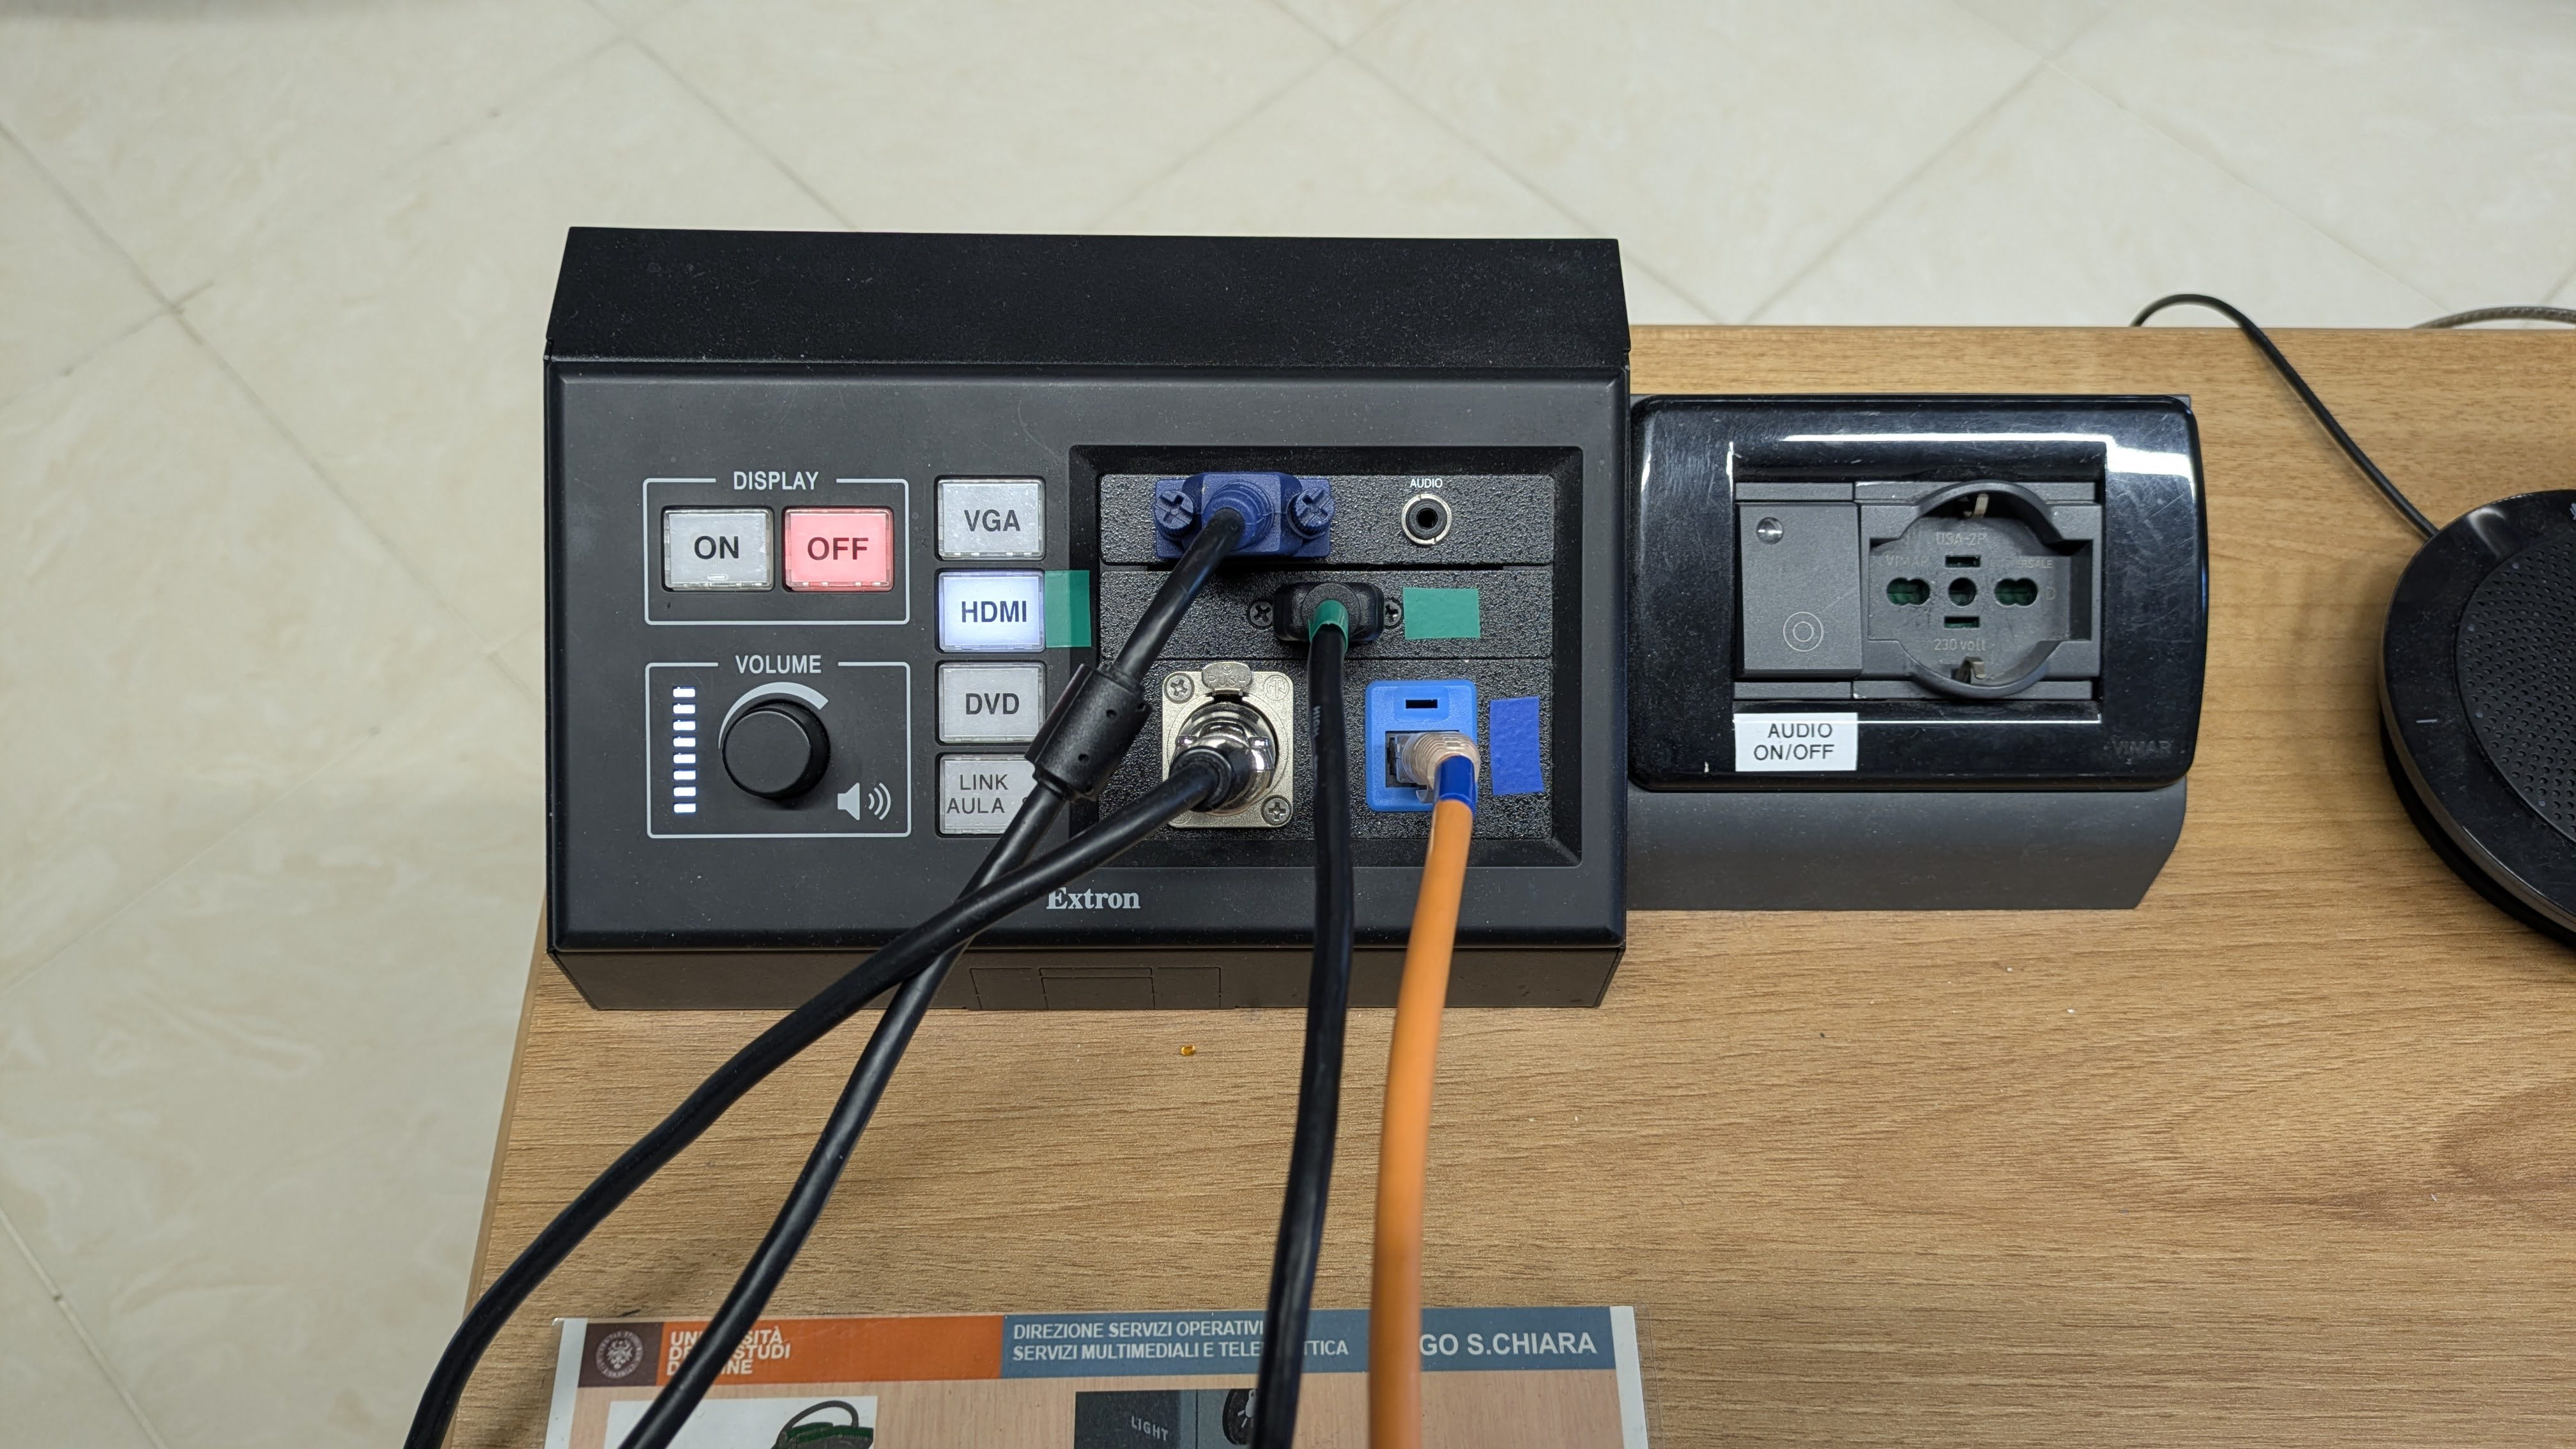
\includegraphics[width=12cm]{imgs/ControllerExtron.jpg}
                \caption{\textit{Controller Multimediale Extron}}
                \label{fig:extron}
            \end{figure}

            \hfill
            \begin{figure}[htbp]
                \centering
                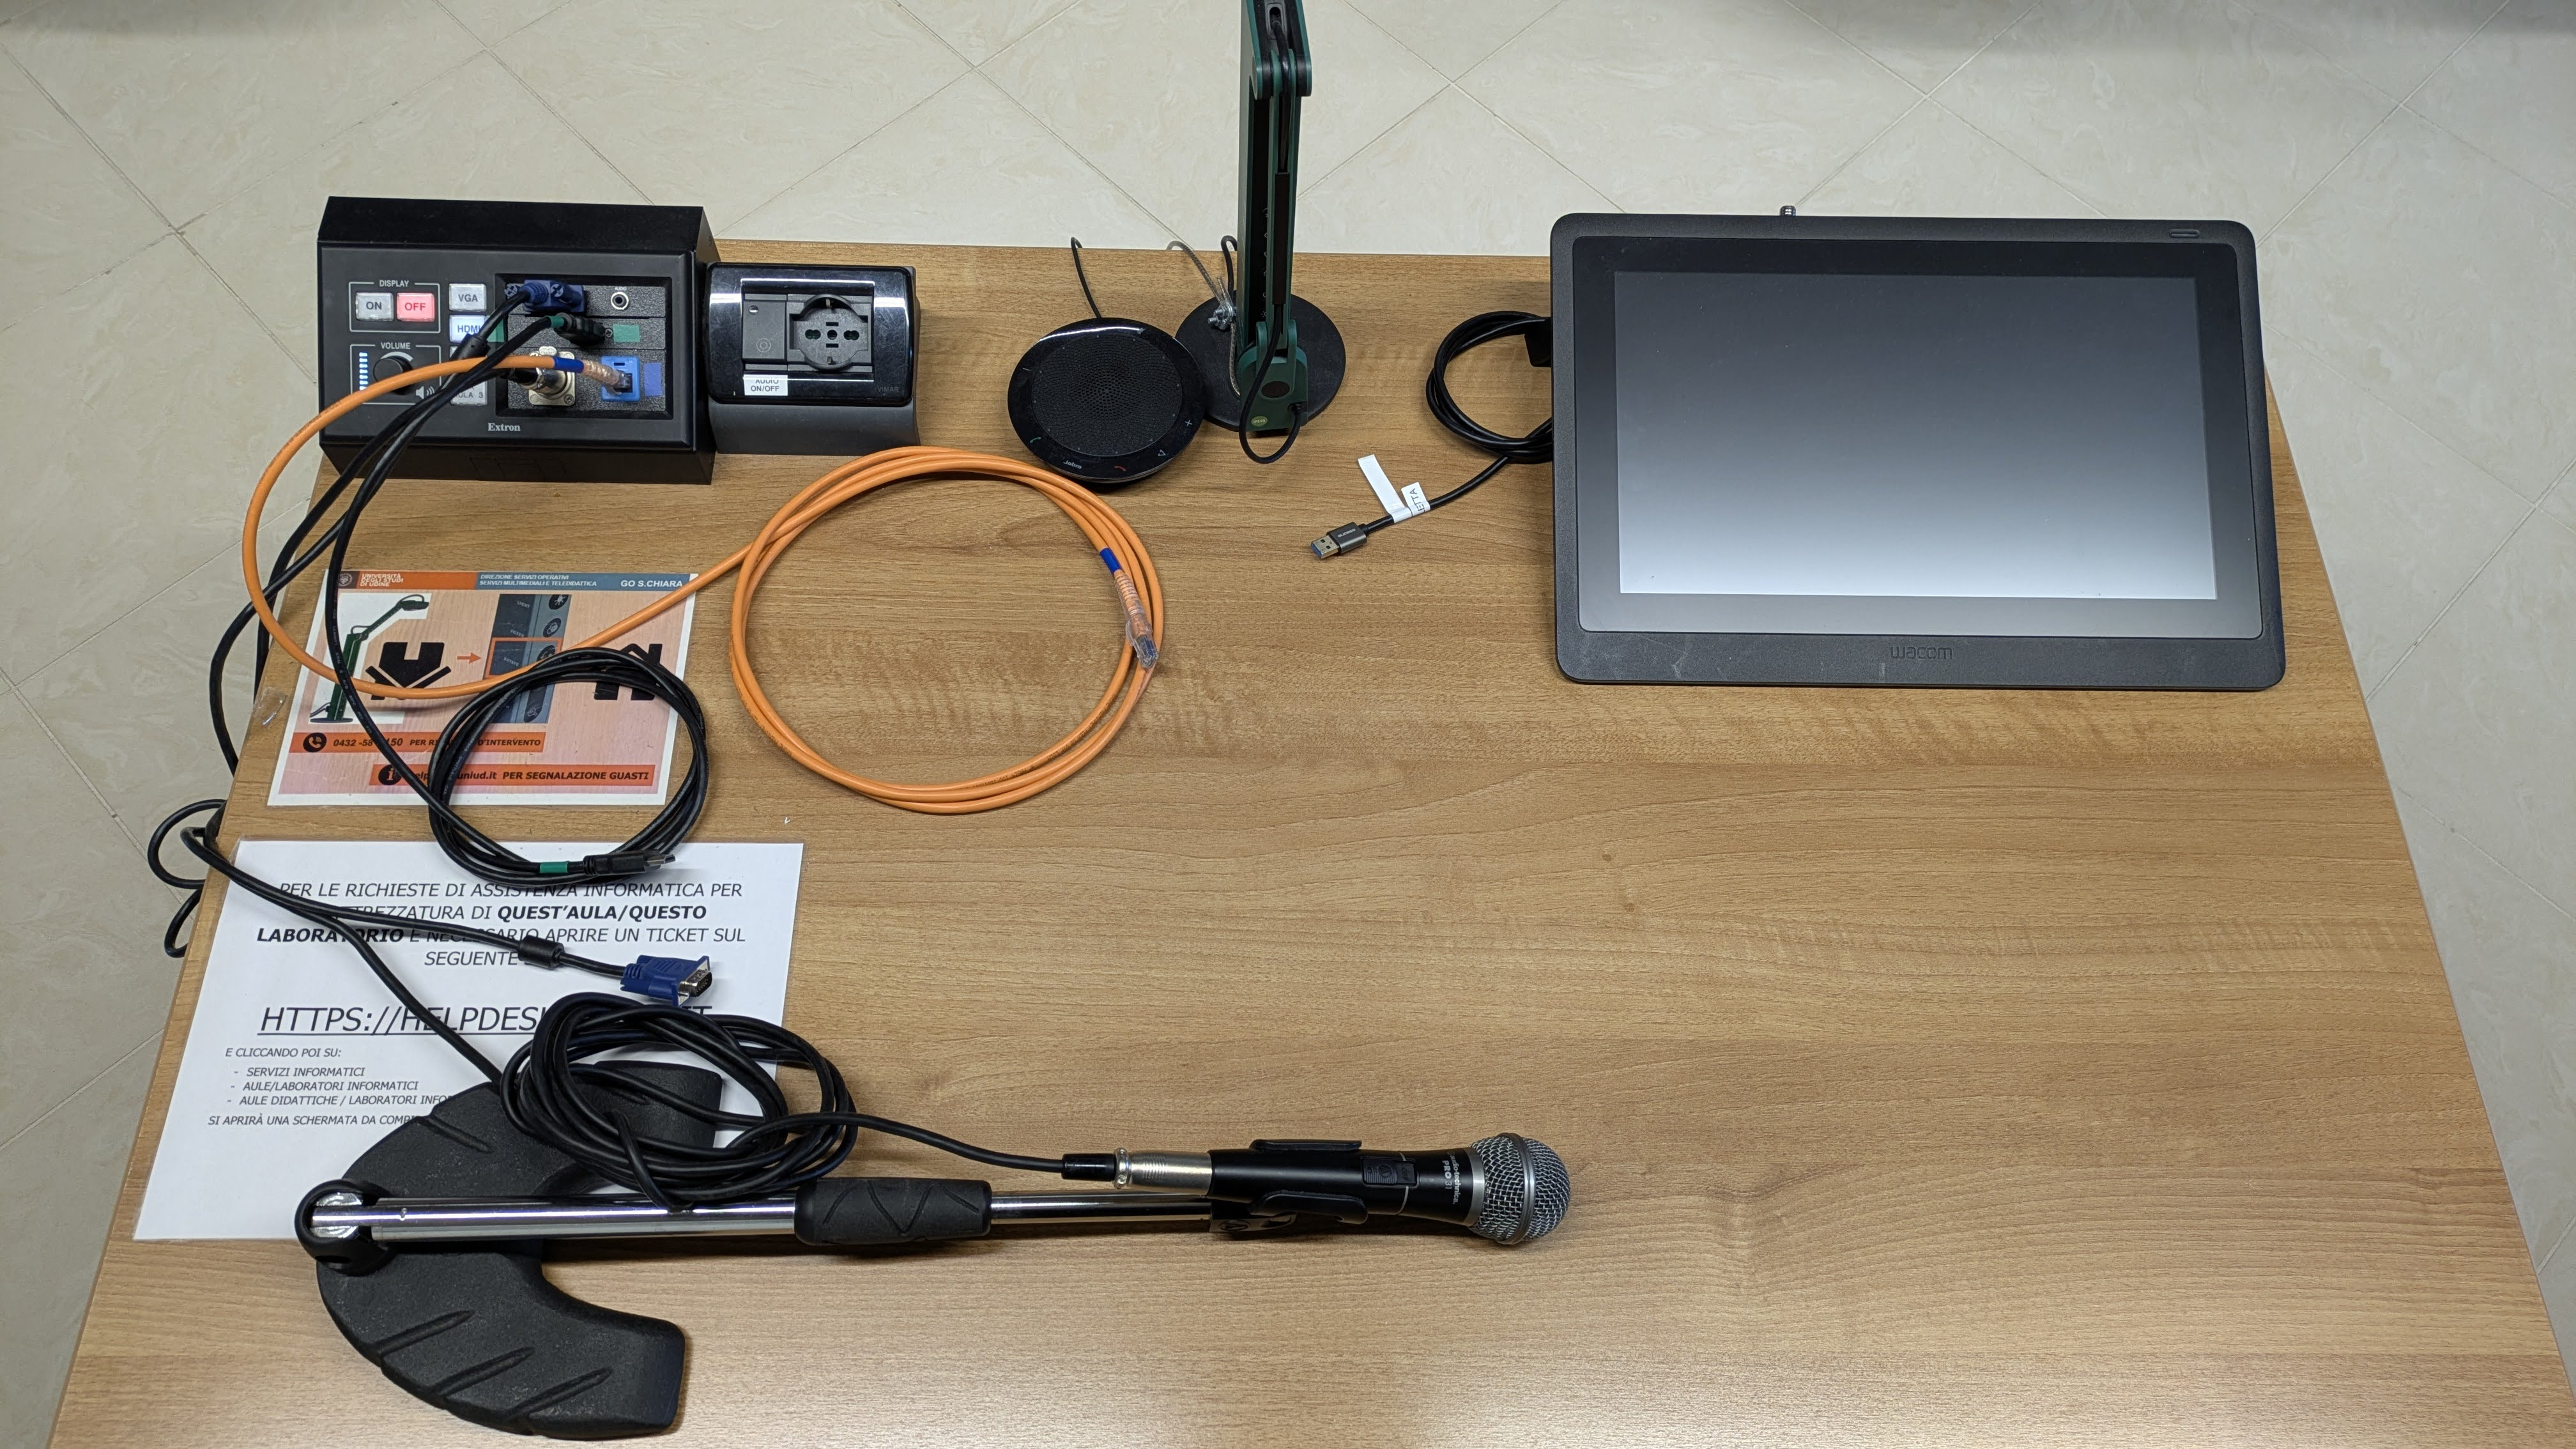
\includegraphics[width=12cm]{imgs/PostazioneDocente.jpg}
                \caption{\textit{Postazione docente delle aule multimediali}}
                \label{fig:postazioneDocente}
            \end{figure}
% ---------------------------------------------------------------------------------------
    \newpage
        \subsubsection{Collegamento Tipo all'impianto Multimediale}
            \par
                Nella seguente procedura non è contemplata la tipologia del computer preso in carico da parte del Docente, in quanto il sistema operativo di riferimento non influisce sulla qualità del servizio multimediale offerto. 
            \par
                L'accensione dell'impianto avviene tramite il tasto "ON" presente nel pannello frontale del controller e tramite la tecnica PoE accende il proiettore. Per il collegamento alla sorgente video, l'Università preferisce l'uso di cavi HDMI rispetto ai cavi VGA in quanto offrono una maggiore compatibilità e un'unica soluzione che comprende audio e video; entrambi però permettono di trasmettere in alta definizione in modalità progressiva (1080p)\footnote{\cite{HDMI22Specification}; "Le principali periferiche", "La gestione delle periferiche", \cite{sciutoIntroduzioneAiSistemi2022}}. 
            \par
                Per eseguire l'accesso ad Internet e poter navigare liberamente, sono necessarie le proprie credenziali Istituzionali. Il sistema distingue il login per studenti (\emph{spes.uniud.it}) da quello del personale interno e dei Docenti (\emph{uniud.it}). \newline
                La pagina di re-indirizzamento al login è basata sul protocollo HTTP, in quanto ha il solo scopo di presentare la prima richiesta alla pagina finale. Una volta che questa comunicazione avviene in qualche istante, bisogna inserite le credenziali e, indipendentemente dalla tipologia di utente autenticato, la comunicazione avviene solamente tramite il protocollo HTTPS in modo da poter trasmettere i vari messaggi in maniera sicura e crittografata attraverso la rete tramite i protocolli \textit{Secure Socket Layer} (SSL) oppure \textit{Transport Layer Security} (TLS). Entrambe le tecniche di crittografia sono valide per il protocollo HTTPS ma non sono interscambiabili (\textit{Figura 3.3}). Sia SSL che TLS permettono e garantiscono diverse proprietà che rendono sicuro il protocollo HTTP, queste sono: 
                \begin{itemize}
                    \item Negoziazione dei parametri: computer e server concordano quali algoritmi crittografici utilizzare.
                    \item Autenticazione del server: Il browser verifica l'identità del sito web tramite un certificato digitale.
                    \item Comunicazione segreta (Riservatezza): I dati vengono cifrati in modo che solo le due parti possano leggerli.
                    \item Protezione dell'integrità: Viene garantito che i dati non vengano manomessi durante il trasporto. 
                \end{itemize}
                Il computer avvia la comunicazione tramite un metodo \textit{handshake} che permette lo scambio delle chiavi crittografiche asimmetriche e, successivamente, la generazione delle chiavi utili alla creazione delle chiavi simmetriche\footnote{"Sicurezza del livello trasporto", \cite{tanenbaumRetiDiCalcolatori2011}}. \newline

            \begin{figure}[htbp]
                \centering
                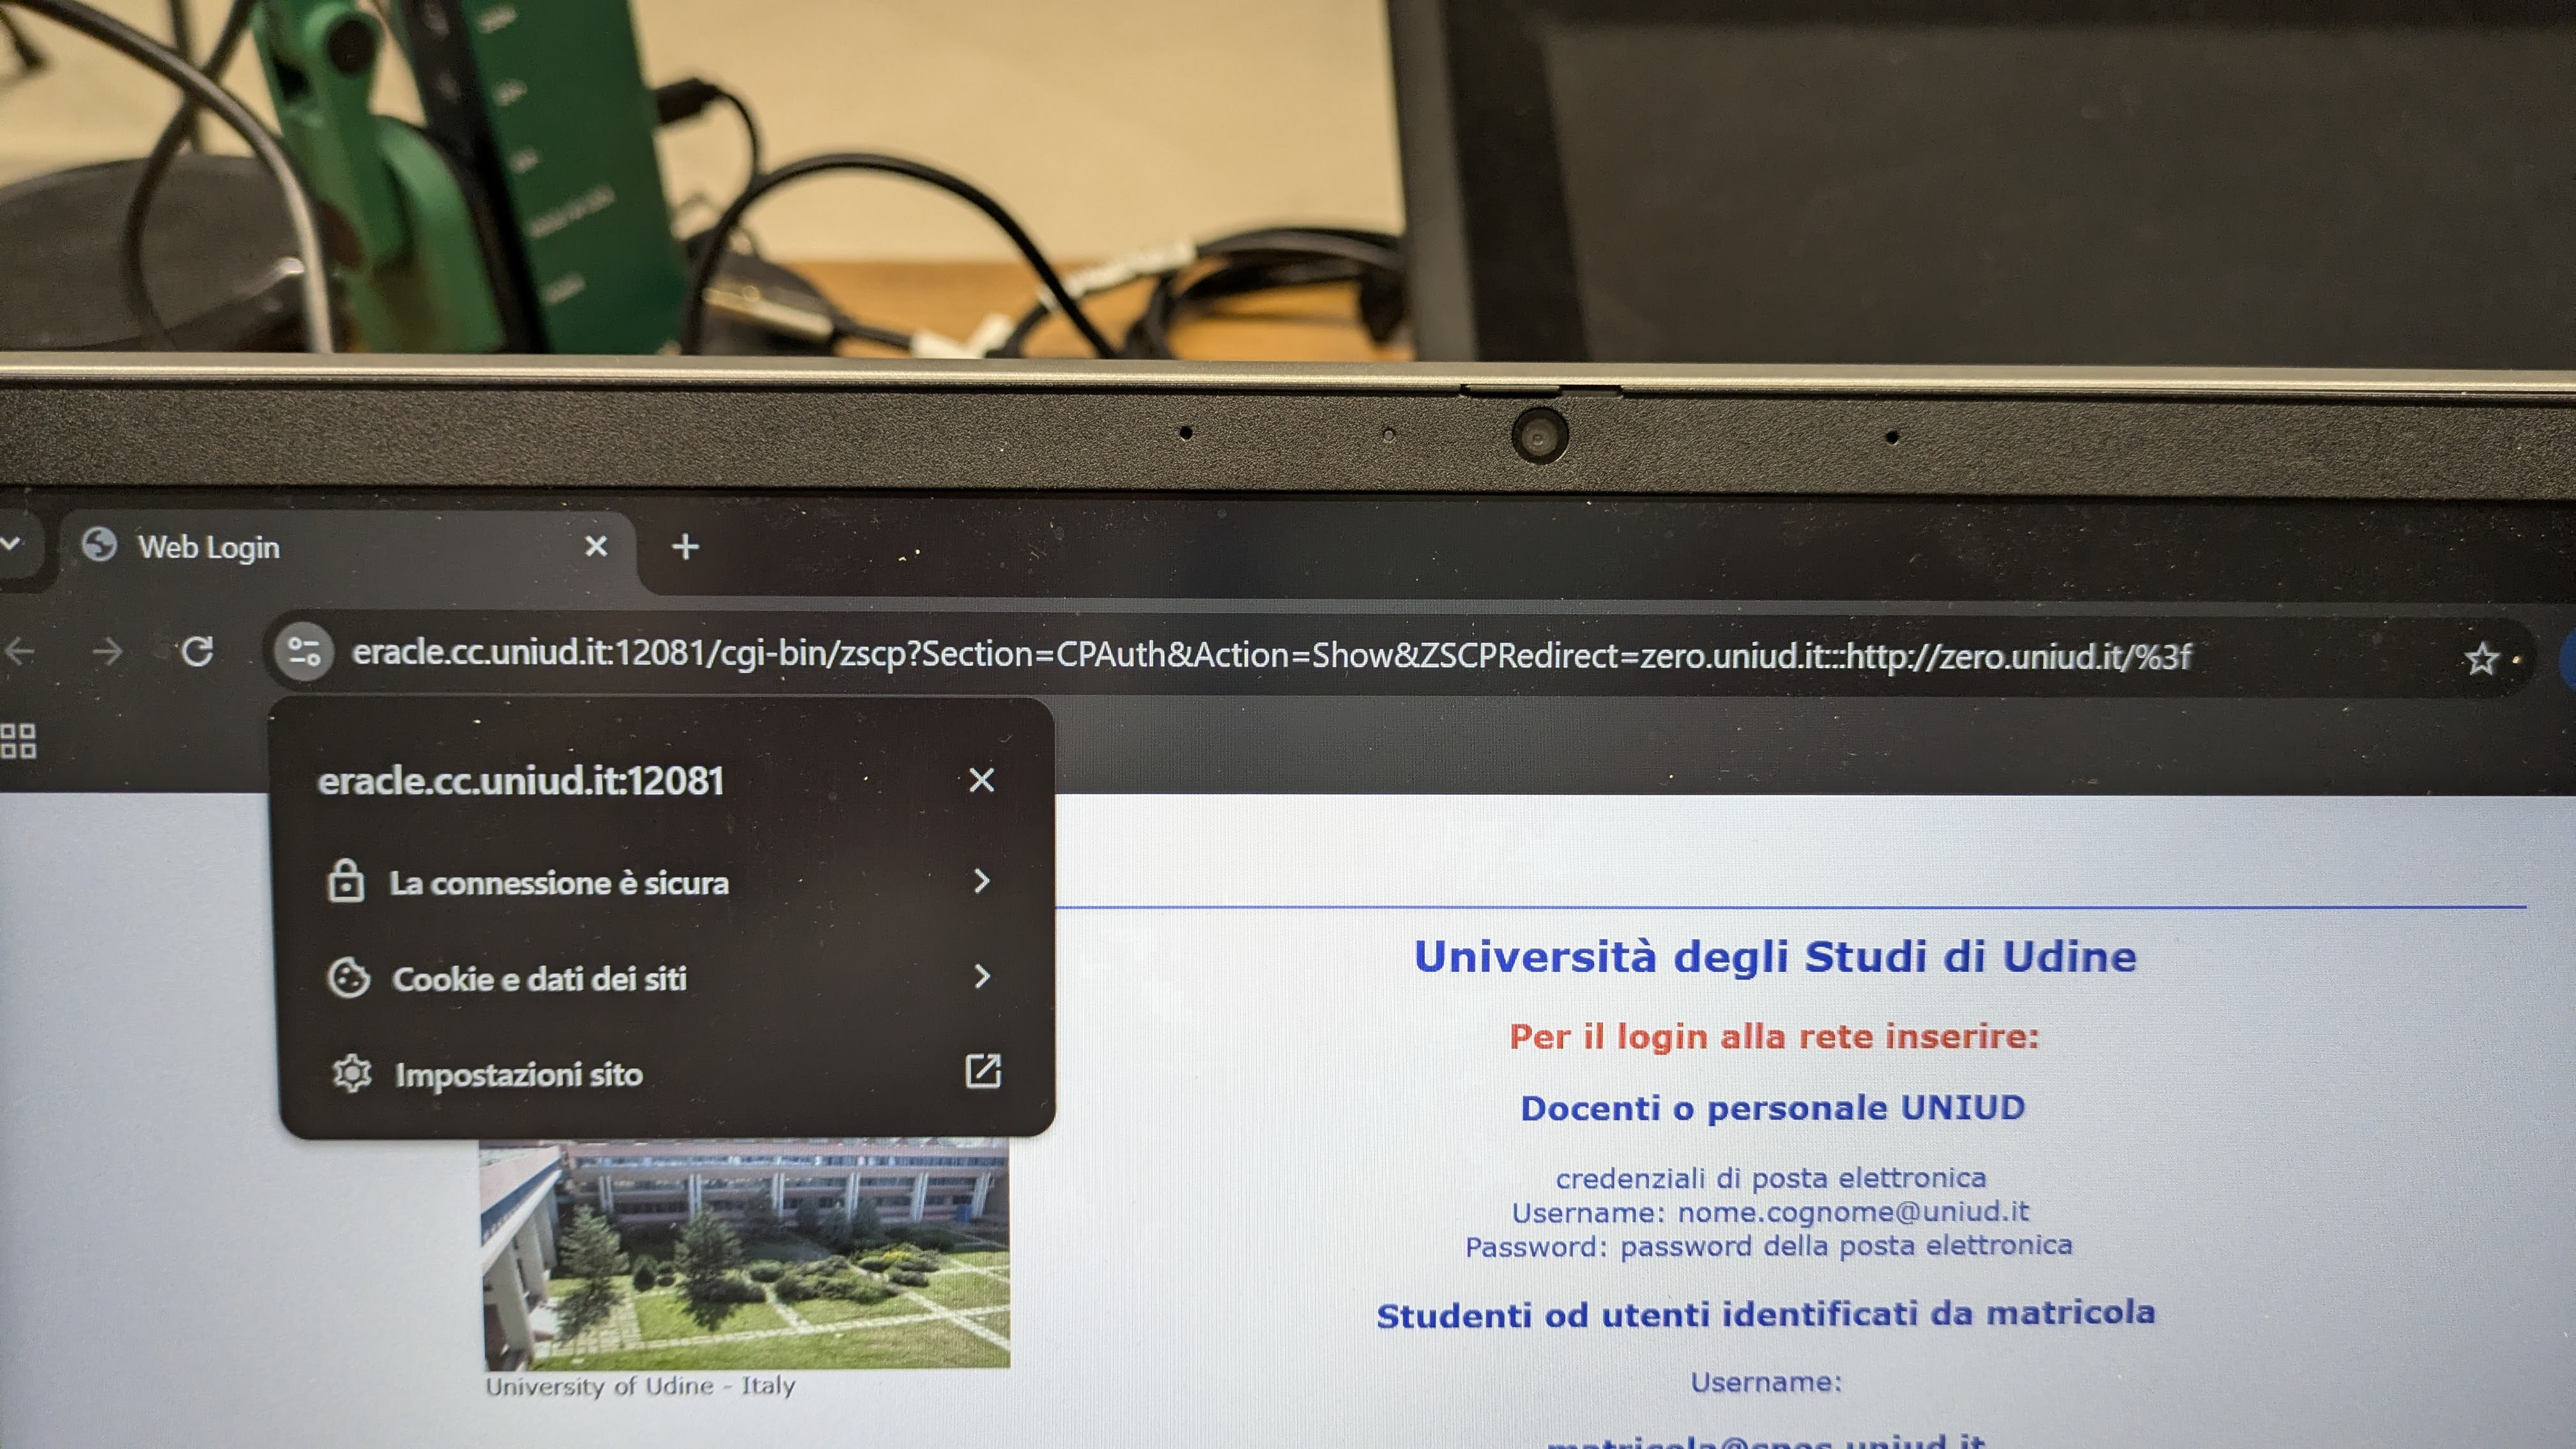
\includegraphics[width=12cm]{imgs/zeroshell.jpg}
                \caption{\textit{Pagina di Login a \emph{zero.uniud.it}}}
                \label{fig:zeroshell}
            \end{figure}

            \par
                Solamente dopo il login con le proprie credenziali si ottiene l'accesso ad Internet per un periodo di tempo determinato; la sessione ha durata diversa in base alla tipologia di account collegato. 
            \par
                L'accesso alla rete Internet non è fondamentale per l'avvio del proiettore tramite il controller \emph{Extron}; su questo controller è possibile trovare diversi tasti che ne regolano il funzionamento, permettendo il comando di altri dispositivi presenti e collegati all'impianto audiovisivo: 
                \begin{itemize}
                    \item Casse stereo; 
                    \item Amplificatore;
                    \item Microfoni direzionali.
                \end{itemize}
                Come descritto in precedenza, il controller Extron presenta un encoder digitale rotativo che permette il controllo preciso del volume in uscita dalle casse stero in dotazione alle aule. Inoltre, solitamente, presenta tre pulsanti dedicati alla gestione delle uscite video e audio ad esso collegate: due uscite HDMI e un'uscita VGA con jack audio da 3.5 mm. Le uscite audiovideo sono reciprocamente esclusive in quanto è impossibile mostrare una sorgente video che non sia stata selezionata dal pannello di controllo. Mentre il proiettore arriva a temperatura e inizia a funzionare, si abbassa il telo bianco dove poi si andrà a proiettare la sorgente video.
            \par
                Nelle aule sono presenti anche dei microfoni direzionali \textsl{gooseneck} o \textsl{cono gelato}; alcuni di questi sono wireless, altri sono cablati. Questi microfoni hanno al loro interno un tasto per poter bloccare la registrazione audio; per ridondanza il controller multimediale presenta un pulsante toggle "audio on/off" o "mute" che non solo blocca la registrazione da parte dei microfoni ma anche la riproduzione audio dalle casse stereo presenti in aula, "spegnendo" completamente il volume fino al prossimo click o alla chiusura dell'impianto (\textit{Figura 3.1}). 
            \par
                Il controller qui riportato è il dispositivo più comune presente nelle aule, tuttavia è presente una sua controparte touchscreen presso l'aula dell'Auditorium Fogar ma il funzionamento è pressoché identico, la sola differenza è la mancanza di un'interfaccia fisica. 
            \par
                Va posta particolare attenzione all'accensione dell'impianto stesso in quanto nella maggior parte dei casi esso viene acceso all'apertura del Centro Polifunzionale; nel caso tuttavia non fosse così, ogni aula ha a disposizione un interruttore che ne controlla accensione e spegnimento. Alcune di queste aule presentano anche un interruttore che, se tenuto premuto, abbassa manualmente il telo del proiettore (\textit{Figura 3.4}); entrambi gli interruttori sono etichettati per distinguerli dalle luci al neon a soffitto. 
                \newline

                \begin{figure}[htbp]
                    \centering
                    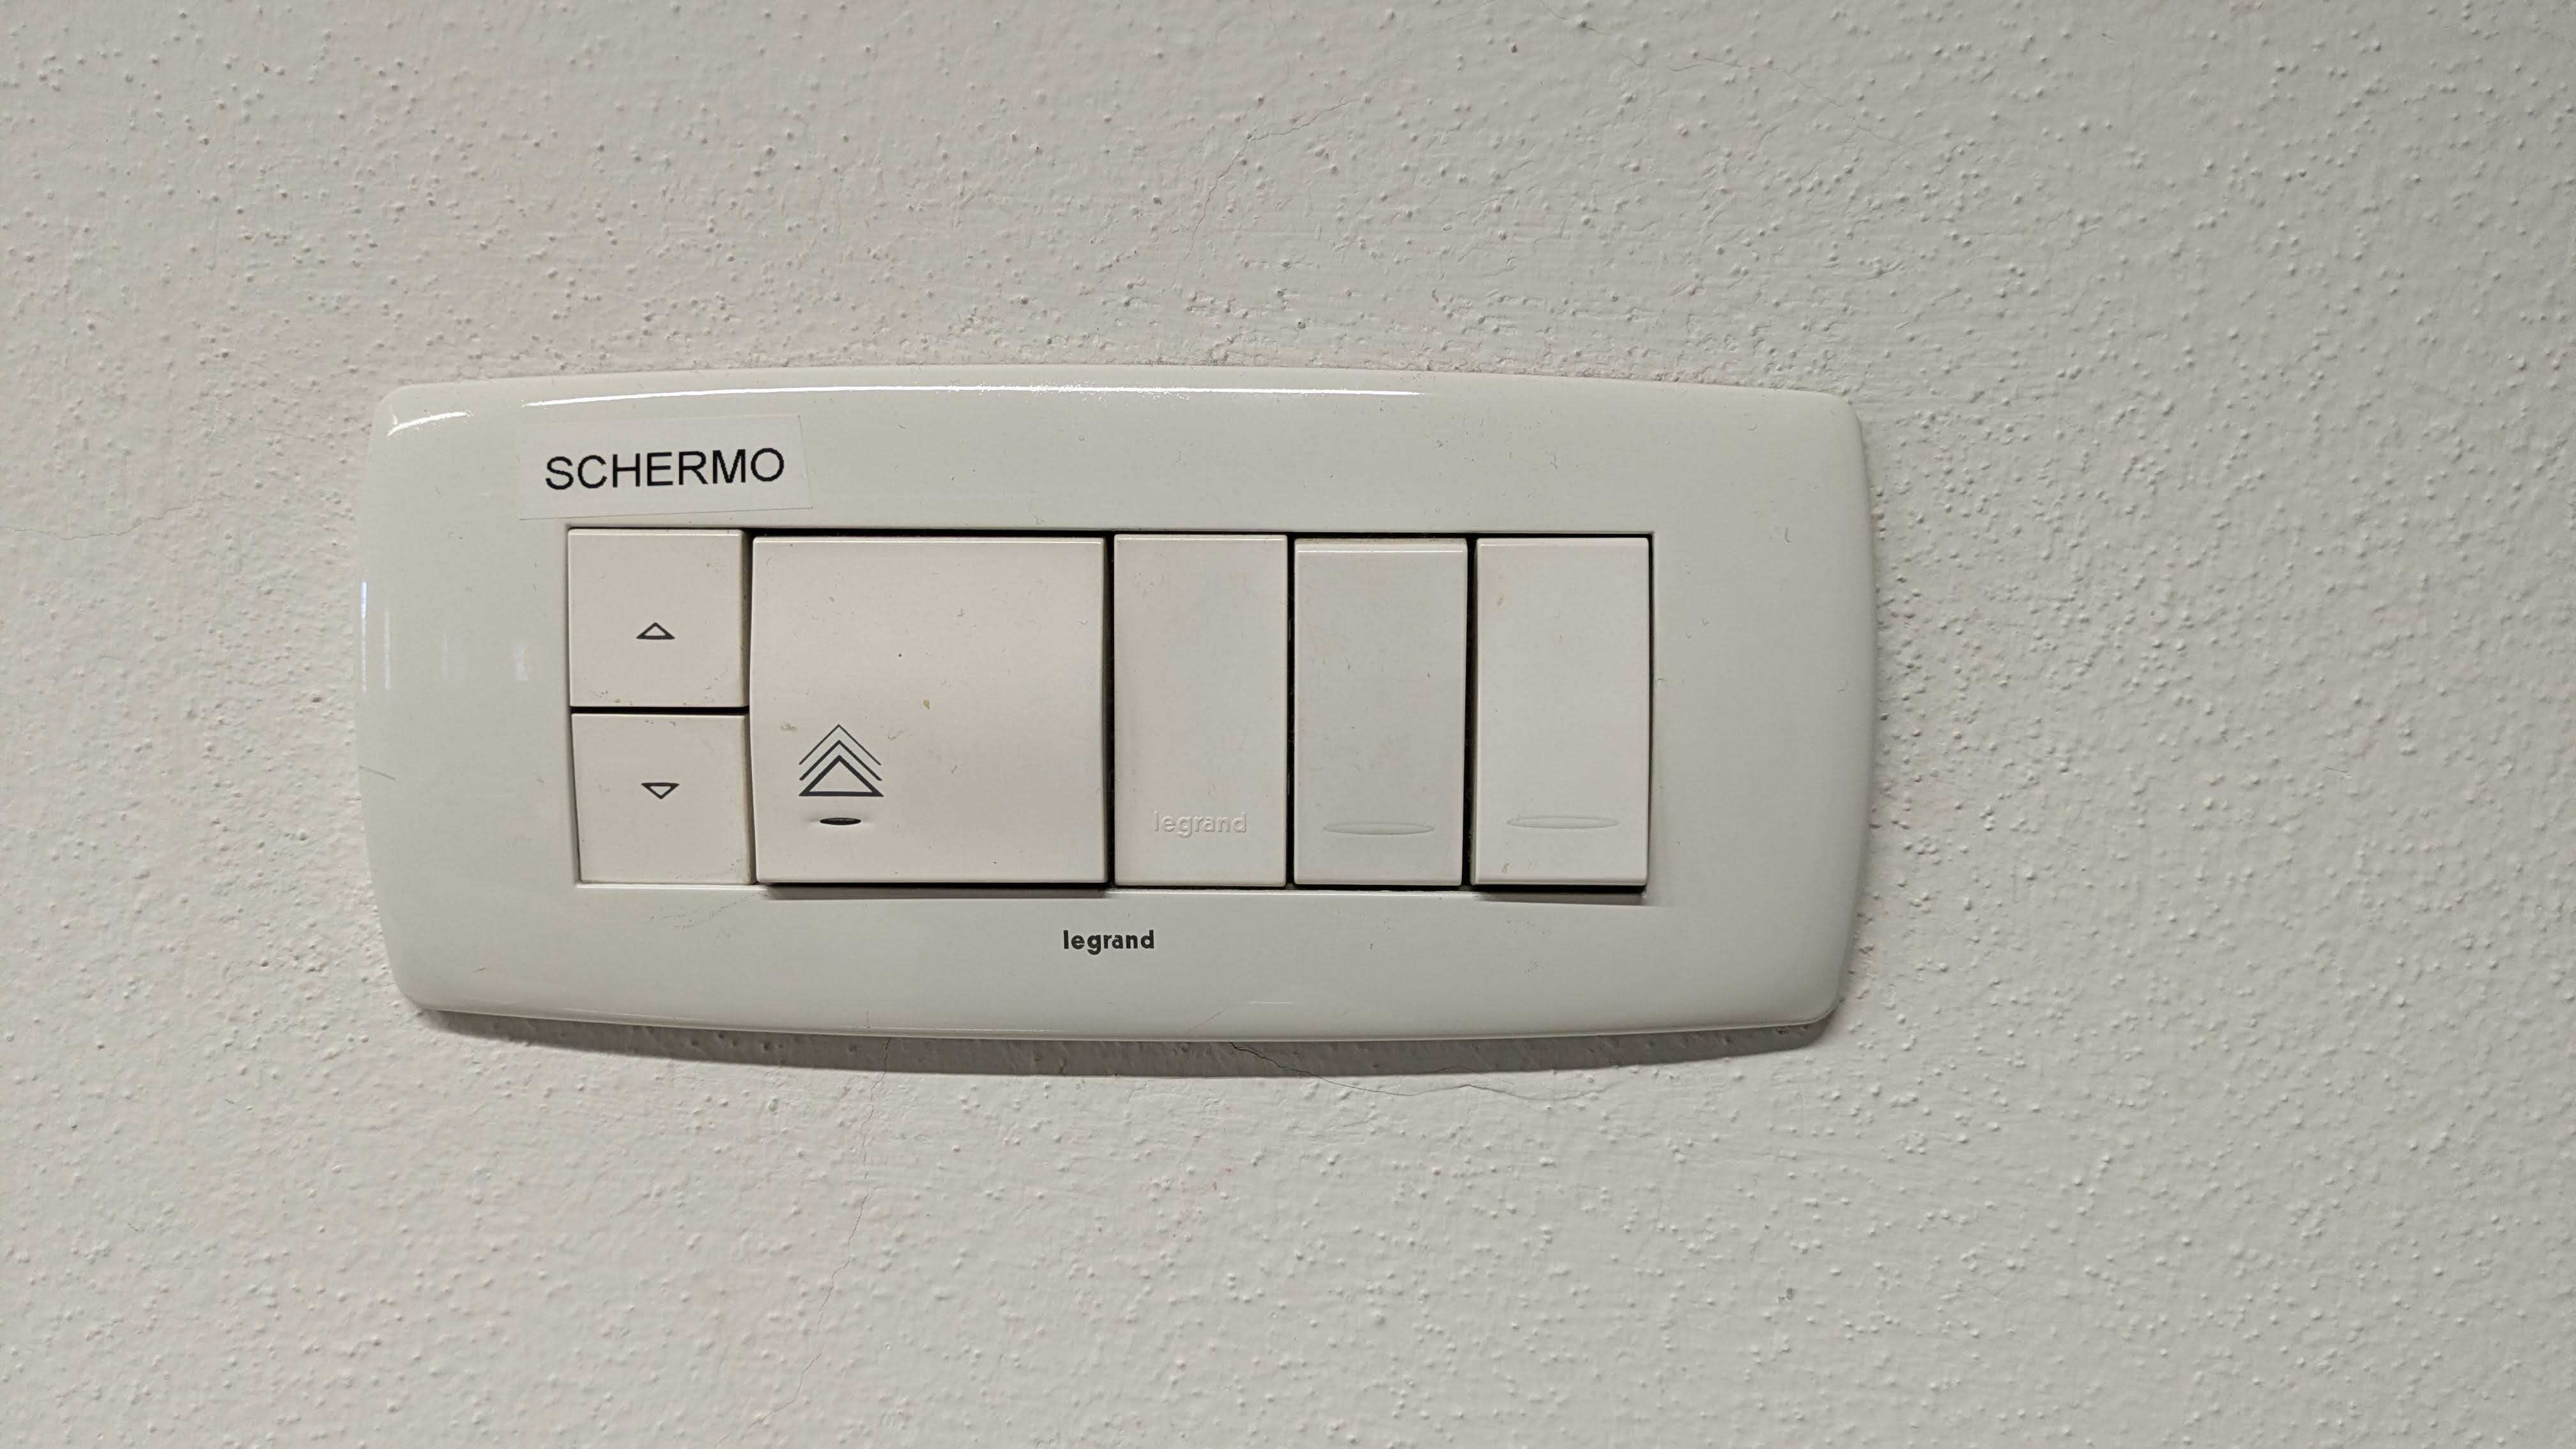
\includegraphics[width=12cm]{imgs/InterruttoriProiettore.jpg}
                    \caption{\textit{Interruttore per il controllo luci e proiettore}}
                    \label{fig:lightswitch}
                \end{figure}
                
            \par
                Il CEGO presenta anche un locale tecnico denominato "Centro Stella" dove si concentrano tutti i servizi TIC offerti dal server della Direzione e il router principale, nonché il collegamento alla backbone o dorsale che permette di interfacciarsi alla Rete di Ateneo. \newline
                All'interno del Centro Stella si possono trovare un server con diversi protocolli e servizi disponibili e un  \textit{Network Attached Storage} (NAS) per l'archiviazione di file e documenti, disponibile e accessibile in rete. 
            \par
                Il server presente all'intero del Centro Stella è stato configurato sulla base della distribuzione Linux Zeroshell. 
                Questa distribuzione è fortemente centrata sulle tecniche di routing e di bridging tra reti, permettendo una connessione completa senza soluzioni di continuità, pur mantenendo un notevole livello di sicurezza. \newline
                Tra i molteplici servizi che offre questa distribuzione Linux possiamo trovare: 
                \begin{itemize}
                    \item il servizio FTP: servizio dedicato allo scambio di file in modo da potervi accedere da qualsiasi postazione della Direzione, si interfaccia con il dispositivo NAS;
                    \item il servizio di Captive Portal: servizio che cattura tutto il traffico di rete e lo reindirizza ad una pagina  di autenticazione;
                    \item il servizio di Autenticazione RADIUS (\textit{Remote Authentication Dial-In User Service}): servizio che gestisce le credenziali di accesso degli utenti \emph{spes.uniud.it} e \emph{uniud.it};
                    \item il servizio Kerberos: servizio che permette l'autenticazione \textit{single sing-on} senza mai far trasmettere la password dell'utente in chiaro attraverso la rete;
                    \item il servizio Certification Authority: servizio che premette la validazione di certificati e firme digitali secondo lo standard X.509 v3, standard utilizzato per la trasmissione delle chiavi pubbliche;
                    \item il servizio Firewall: servizio mirato alla sicurezza filtrando l'accesso alla rete di virus e utenti malevoli;
                    \item il servizio di VPN: servizio che permette di configurare una rete privata virtuale, sia \textit{Host-to-LAN} che \textit{LAN-to-LAN};
                    \item il servizio VLAN Mapping: servizio che supporta lo standard IEEE 802.1Q, ovvero la creazione di più VLAN su specifici; 
                    \item il servizio QoS: servizio ormai presente su qualsiasi dispositivo di rete moderno, permette di bilanciare diversamente le varie tipologie di traffico di rete per garantire la migliore qualità di trasmissione. 
                \end{itemize}
                Il servizio FTP è un servizio progettato per permettere lo scambio di file e dati tra due o più computer o tra un computer e un server, creando una sorta di tunnel virtuale per l'\textit{upload} e successivo \textit{download} del file. In aggiunta a \textit{Zeroshell} si possono configurare funzioni aggiuntive di filtraggio e di monitoraggio degli accessi, ottimizzandone il recapito\footnote{"QoS and Traffic Shaping", \cite{ZeroshellLinuxRouter2021}}.
            \par
                Il servizio di Captive Portal funge da "rete di cattura" per tutto il traffico Internet, reindirizzando tutte le richieste ad una pagina di autenticazione, impostata dal pannello di controllo del server, in modo da accreditare ogni utente connesso. Le credenziali vengono controllate dal Captive Portal tramite il server RADIUS/Kerberos.
                \footnote{"Hotspot using Captive Portal", \cite{ZeroshellLinuxRouter2021}}
            \par
                Il servizio di autenticazione RADIUS permette una centralizzazione dell'autenticazione in un unico server, semplificando e alleggerendo il lavoro dei vari punti di accesso ospitando il database, o parte di esso, delle credenziali di accesso. Il servizio è stato idealizzato per reti cablate ma è utilizzato anche per le connessioni wireless\footnote{"Wireless e reti mobili", "Sicurezza nelle reti", \cite{kuroseRetiDiCalcolatori2022}} come può esserlo la rete di Ateneo \textit{Eduroam}.
            \par
                Il servizio di autenticazione Kerberos premette di autenticarsi in rete, come RADIUS, solamente con una tecnica diversa in quanto necessita di tre entità per poter creare una comunicazione sicura: l'\textit{Authentication Server} (AS), il \textit{Ticket-Granting Server} (TGS) e il server a cui si vuole accedere. Questa architettura permette l'inserimento della propria password solamente una singola volta e questa non verrà mai trasmessa in chiaro sulla rete. Entrando nei dettagli tecnici, questo protocollo lavora sugli orologi di sistema dei dispositivi, richiedendo che questi siano sincronizzati a quello del TGS. Il messaggio cifrato contenente i vari dati per la configurazione della comunicazione sicura è costruito attorno al messaggio che manda il TGS e quindi non è facilmente intercettabile da utenti terzi. Grazie a questa caratteristica architettonica del protocollo, è possibile scalare i servizi disponibili, predisponendo diversi reami con più AS, TGS e servizi a cui si vuole accedere\footnote{"Autenticazione con Kerberos", \cite{tanenbaumRetiDiCalcolatori2011}; "LDAP directories" \cite{ZeroshellLinuxRouter2021}}. 
            \par
                Il servizio di Certification Authority (CA) permette di autenticare in modo sicuro l'utente connesso e, soprattutto, ne garantisce l'univocità tramite la creazione di un certificato di sicurezza contenente la rispettiva chiave pubblica. Questi certificati sono firmati digitalmente da un algoritmo, scelto durante la fase di configurazione, e possono essere rinnovati o revocati. Per poter confermare un utente sconosciuto, il suo certificati viaggia per una catena di diverse CA fino alla Root CA, nel caso dell'Università di Udine è ipotizzabile che la Root CA si trovi all'interno della sede centrale d'Ateneo. \newline
                La conferma dei certificati di sicurezza è fondamentale per poter garantire una comunicazione sicura, sono omessi ma presenti nei dati tecnici di molti algoritmi sicuri tra cui SSL, TLS e le VPN\footnote{"Authentication on Wireless networks with 802.1x, WPA and WPA2", "Virtual Private Network (VPN)", "Virtual Private Network (VPN)", \cite{ZeroshellLinuxRouter2021}}. 
            \par
                Il servizio Firewall è fondamentale se si vuole proteggere la rete interna all'Università da attacchi malevoli mirati all'interruzione di servizio. Il firewall filtra tutto il traffico in entrata e in uscita dalla rete LAN in base a delle regole precedentemente configurate. Zeroshell integra anche un sistema di protezione dagli attacchi \textit{Denial of Service} (DoS)\footnote{"Firewall SPI and Packet Filter", \cite{ZeroshellLinuxRouter2021}}.
            \par
                Il servizio VPN permette di aggiungere flessibilità all'accesso di rete, permettendo di collegarsi alla rete LAN anche se non si è presenti fisicamente al suo interno. Questa connessione è creata tramite una rete virtuale privata, garantendo l'accesso autenticato al dispositivo inserito\footnote{"Virtual Private Network (VPN)", \cite{ZeroshellLinuxRouter2021}}. Questa tecnica è utilizzata per poter accedere da remoto al server NAS con i portatili in uso dalla Direzione. 
            \par
                Il servizio VLAN Mapping permette di far corrispondere reti VLAN a specifici identificativi di reti wireless in modo da gestire permessi e livelli di sicurezza diversi in base alle esigenze delle VLAN. È possibile creare un'assegnazione dinamica interfacciandosi con il servizio RADIUS oppure mappare manualmente le varie reti inserendo bridge virtuali che contrassegneranno il traffico come se fosse diretto a quella rete\footnote{"Wireless Access Point with Multiple SSID and VLAN Mapping", \cite{ZeroshellLinuxRouter2021}}. 
            \par
                Il servizio QoS ha un'architettura simile al servizio di firewall, in quanto filtra e monitora tutto il traffico che attraversa la rete. Questo monitoraggio è svolto con l'obiettivo di garantire i giusti pesi ai vari pacchetti che transitano in rete, per esempio offrendo una maggiore banda agli applicativi \textit{Voice-over-Internet-Protocol} (VoIP)\footnote{"QoS and Traffic Shaping", \cite{ZeroshellLinuxRouter2021}}. 